\chapter{Dynamic Query Expansion}
\markright{Aravindan Mahendiran \hfill Chapter 2. Dynamic Query Expansion\hfill}
\section{Query Expansion}
In most document corpora, a single concept can be referred using multiple terms.
In information retrieval (IR) this is called \emph{synonymy} and has a huge impact on the recall of documents pertaining to the concept.
Researchers address this problem by creating as exhaustive a query as possible. 
But when exploring the Twitter corpora it becomes almost impossible to hand craft such a expansive query as the meme and hash-tag adaptations are not known a priori. 
\newline
To address this issue IR experts use \emph{query expansion} or reinforcement learning.
These are iterative algorithms that are initialized with a small set of query terms. 
When the documents matching the query terms are returned, after basic  processing such as tokenization, stop-word removal and stemming a richer vocabulary is obtained by ranking the terms in these documents by their frequency counts.
The top words from this list is then used to query the documents again. 
This process goes on until no new terms are added to the vocabulary. 
We design and implement such an pipeline using Probabilistic Soft Logic to build our vocabulary for a given election. 
We first review the PSL framework before proceeding to detail our methodology.
\section{Probabilistic Soft Logic}
Probabilistic Soft Logic ~\cite{kimmig2012short} is a framework for collective probabilistic reasoning on relational domains.
PSL models have been developed in various domains, including collective classification ~\cite{broecheler2010computing}, ontology alignment ~\cite{brocheler2012probabilistic}, personalized medicine ~\cite{bach2010decision}, opinion diffusion ~\cite{bach2012scaling} , trust in social networks ~\cite{huang2012probabilistic}, and graph summarization ~\cite{memory2012graph}.
PSL represents the domain of interest as logical atoms.
It uses first order logic rules to capture the dependency structure of the domain, based on which it builds a joint probabilistic model over all atoms.
Instead of hard truth values of $0$ (false) and $1$ (true), PSL uses soft truth values relaxing the truth values to the interval $[0,1]$.
The logical connectives are adapted accordingly.
This makes it easy to incorporate similarity or distance functions.
\newline
User defined \emph{predicates} are used to encode the relationships and attributes and \emph{rules} capture the  dependencies and constraints.
Each rule's antecedent is a conjunction of atoms and its consequent is a dis-junction. 
The rules can also labeled with non negative weights which are used during the inference process. 
The set of predicates and weighted rules thus make up a PSL program where known truth values of ground atoms are set from observed data and unknown truth values for the remaining atoms are learned using the PSL inference mechanism.
\newline
Given a set of atoms 
$\ell = \{\ell_1,\ldots,\ell_n\}$,
an interpretation defined as 
$I : \ell \rightarrow [0,1]^n$
is a mapping from atoms to soft truth values.
PSL defines a probability distribution over all such interpretations such that those that satisfy more ground rules are more probable.
\emph{Lukasiewicz t-norm} and its corresponding co-norm are used for defining relaxations of the logical AND and OR respectively to determine the degree to which a ground rule is satisfied.
Given an interpretation $\mathit{I}$, PSL defines the formulas for the relaxation of the logical conjunction ($\wedge$), dis-junction ($\vee$), and negation ($\neg$) as follows:

\begin{align*}
\ell_1 \softand \ell_2 &= \max\{0, I(\ell_1) + I(\ell_2) - 1\},\\
\ell_1 \softor \ell_2 &= \min\{I(\ell_1) + I(\ell_2), 1\},\\
\softneg l_1 &= 1 - I(\ell_1),
\end{align*}  
where we use \textasciitilde to indicate the relaxation of the Boolean domain.
The interpretation $\mathit{I}$ determines whether the rules is satisfied, if not, the \emph{distance to satisfaction}.
A rule $\mathit{r} \equiv \mathit{r_{body}} \rightarrow \mathit{r_{head}} $  is satisfied if and only if the truth value of head is atleast that of the body. The rule's distance to satisfaction measures the degree to which this condition is violated.
 \newline
\begin{center} 
 $\mathit{d_r}(\mathit{I}) =$ max\{0,$\mathit{I(r_{body}} - \mathit{I(r_{head}}$\}
 \end{center}

PSL then induces a probability distribution over possible interpretations $\mathit{I}$ over the given set of ground atoms $\mathit{l} $ in the domain. 
If $\mathit{R}$ is the set of all ground rules that are instances of a rule from the system and uses only the atoms in  $\mathit{I}$ then,
the probability density function $\mathit{f}$ over $\mathit{I}$ is defined as
\begin{equation}
\label{eq:contimn1}
    f (I) = \frac{1}{Z} \text{exp}[-\sum_{r\in R} \lambda_r (d_r(I))^p]
\end{equation}
\begin{equation}
\label{eq:contimn2}
	Z = \int_{I} \text{exp} [ -\sum_{r\in R} \lambda_r (d_r(I))^p ]
\end{equation}
where~$\lambda_r$ is the weight of the rule~$r$, $Z$ is the continuous version of the normalization constant used in discrete Markov random fields, and ~$p \in \{1, 2\}$ provides a choice between two different loss functions, linear and quadratic.
The values of the atoms can be further restricted by providing linear equality and inequality constraints allowing one to encode functional constraints from the domain.
\paragraph{}
PSL provides for two kinds of inferences (a)most probable explanation and (b)calculation of the marginal distributions. 
In the MPE inference given a partial interpretation with grounded atoms based on observed evidence, the PSL program infers the truth values for the unobserved atoms satisfying the most likely interpretation. 
In the second setting, given ground truth data for all atoms we can learn the weights for the rules in our PSL program.
In our work we leverage the MPE inference.
\section{Dynamic Query Expansion using PSL}
In ~\cite{huang2012social}, we used PSL to model user affiliations within groups. 
Specifically we built a PSL program for a  social network where we have a set of users, their posts, messages to other users and the various groups we want to model. 
The rules we defined captured the dynamics of group affiliations through the various interactions.
Through the MPE inference we classified users into different groups based on their hash-tag usage and their interactions with other users.
\paragraph{}
In this paper we extend our earlier work to achieve what we call dynamic query expansion through PSL. 
Similar to the query expansion methodology described earlier we start with an initial set of hash-tags which we believe are indicative of the affinity of a particular user to a candidate contesting in the election.
We refer to these hash-tags as seed words.
Instead of a single inference, we iteratively perform the inference over successive time windows such that the inference from window $w_t$ is used as a prior to window $w_{t+1}$ and the inference from that is used for window $w_{t+2}$ and so on.
\begin{figure*}[Ht]
	\centering
	%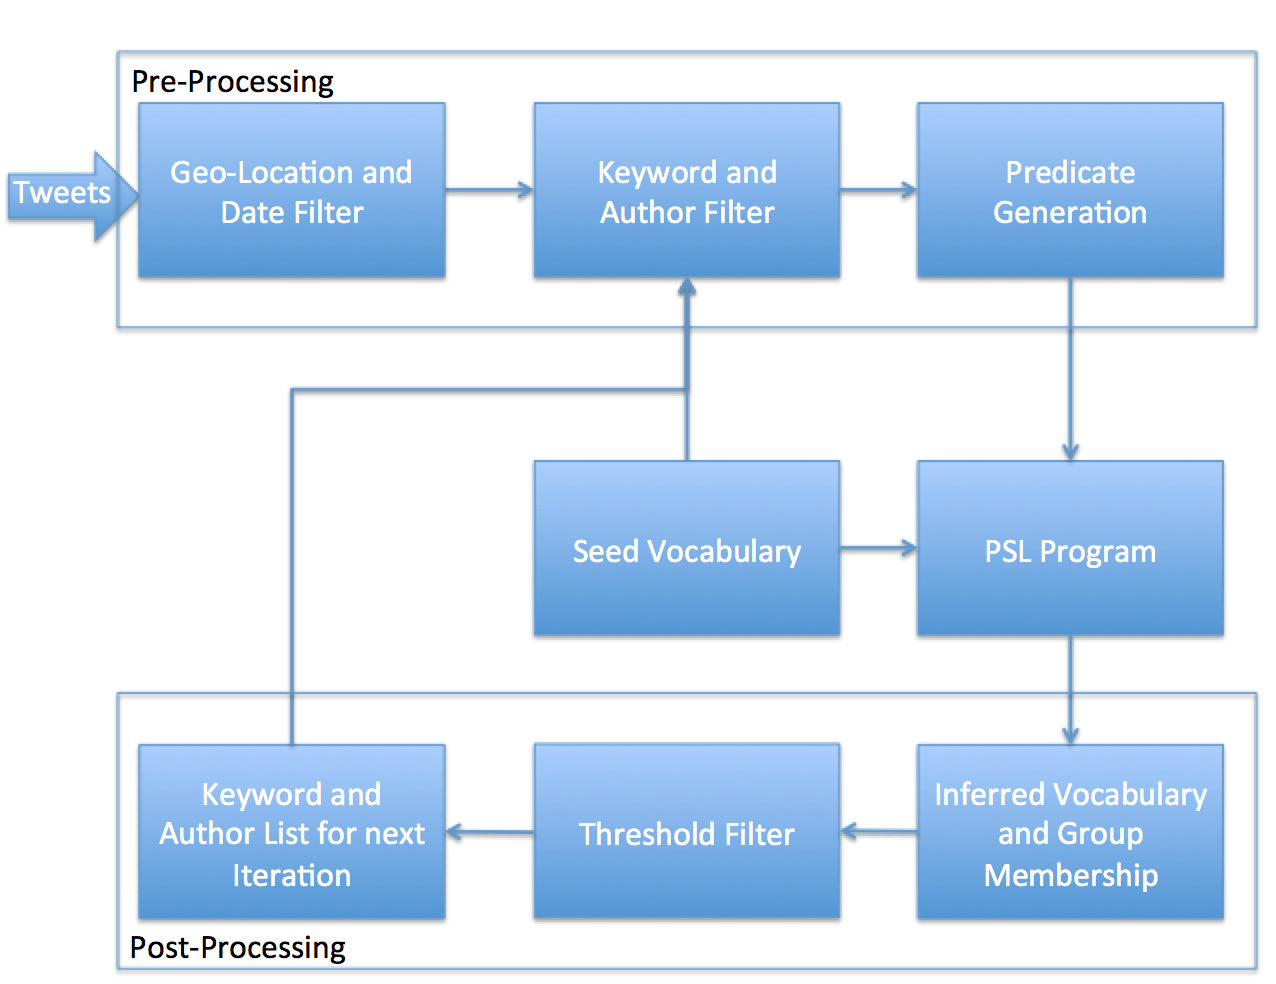
\includegraphics[scale=0.50]{support_files/flowChart.png}
	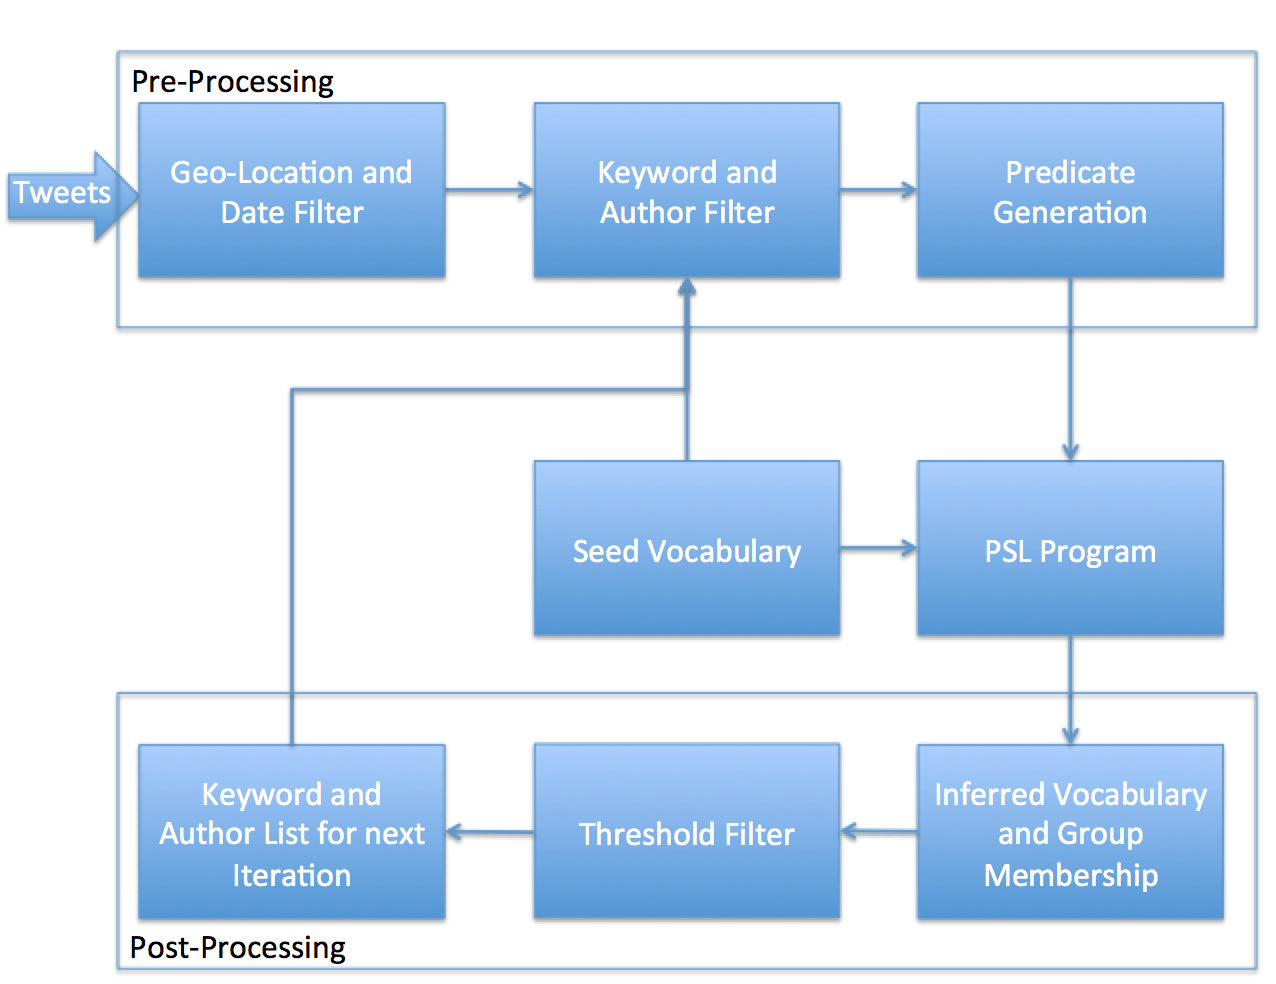
\includegraphics[height=0.5\textheight, width=1.0\textwidth]{support_files/flowChart.png}
	\caption{Design of the query expansion pipeline.}
	\label{fig:flowchart}
\end{figure*}
\paragraph{}
Figure\ref{fig:flowchart} illustrates the design of the iterative algorithm for dynamic query expansion.
The initial pre-processing starts with the tweet input stream which is filtered by the date range specified by the window size. 
For each election, tweets from a month leading up to the election were used.
After extensive analysis it was determined that the most optimal window size was 3 days. 
Smaller window sizes resulted in sub-optimal inferences as there were not enough data points feeding into the PSL stage.
Larger window sizes lead to memory issues as the PSL optimization has a time complexity of  $O(n^{3.5})$ where $n$ is the number of relevant rule groundings, i.e., those with non-zero distance to satisfaction. 
The tweets passing the date filter are then geo-coded using a geo-location algorithm that infers the location of a tweet. 
This ensures that only tweets originating from the country of interest are used.
The geo-location algorithm tags the tweets with a location by looking at the GPS coordinates of the tweet if available or landmarks and locations mentioned in the tweet or author's profile. 
For tweets that do not have either of these information it uses a label propagation algorithm to infer the author's location through his/her network.
\newline
The geo-tagged tweets are then tracked for the presence of a hash-tag from the vocabulary for that particular iteration.
In addition to filtering tweets using the vocabulary the authors whose affiliations are already inferred by the system are also used as a filtering criteria.
The tweets are then converted into PSL predicates and fed into the inference process.
The PSL program infers the hash-tags and tweeters that are mostly associated with a particular candidate. 
Each author and hash-tag's association with a candidate is measured using the truth value of the predicate grounding.
In the post-processing step, these truth values are filtered by a threshold value to identify the hash-tags and authors strongly associated to a candidate.
These hash-tags become a part of the vocabulary of the candidate and along with the users identified are used as a filter criterion for the next iteration.
This iterative process proceeds until the day before the election when we obtain the final vocabulary which are strongly associated with a candidate.
\paragraph{}
Within the PSL program we define predicates to encode the network. 
The predicates $Tweeted(U,T)$ and $Contains(T,W)$  capture the fact that a user $U$ tweeted a tweet $T$ and tweet $T$ contains hash-tag $W$ respectively. 
Similarly, the belief that a user $U$ or hash-tag $W$ is affiliated/associated to the group $G$ is encoded as $Is\_Member(U,G)$ and $Belongs(W,G)$ respectively.
In order to capture the temporal connectivity between the iterations, in addition to the initiating the inference process with the rule
\begin{align*}
Seed\_Word(W,G) \Rightarrow Belongs(W,G)
\end{align*}
we define additional rules such as
\begin{align*}
Was\_Member(A,G) \Rightarrow Is\_Memeber(A,G)
\end{align*}
\begin{align*}
Belonged(W,G) \Rightarrow Belongs(W,G)
\end{align*}
where the predicates $Was\_Member$ and $Belonged$ are inferences from the previous time window and are loaded in as  priors for the current iteration.
These rules are weighted slightly lower than the recursive rules below so that the system overcomes the bias it had learned in light of new more convincing evidence.
This way hash-tags that are more indicative of a user's affiliation are assigned stronger truth values or weights for every successive iteration and the weights hash-tags that aren't are reduced.
The same reasoning applies to the user-candidate affiliations(memberships) too.
Below we outline the recursive PSL rules that grows the hash-tag preferences and the user affiliations. 
\begin{align*}
\begin{split}
Tweeted(A,T) 
	\softand Contains(T,W)
	\softand Belongs(W,G) \\ 
	\softand Positive(T)
	\Rightarrow Is\_Member(A,G)
\end{split}
\end{align*}

\begin{align*}
\begin{split}
Tweeted(A,T)
	 \softand Contains(T,W)
	\softand Belongs(W,G)\\
	 \softand Negative(T)
	\Rightarrow \sim Is\_Member(A,G)
\end{split}
\end{align*}

\begin{align*}
\begin{split}
Is\_Member(A,G)
	 \softand Tweeted(A,T)
	\softand Contains(T,W)\\
	 \softand Positive(T) 
	\Rightarrow Belongs(W,G)
\end{split}
\end{align*}

\begin{align*}
\begin{split}
Is\_Member(A,G) 
	\softand Tweeted(A,T)
	\softand Contains(T,W)\\
	\softand Negative(T)
	\Rightarrow \sim Belongs(W,G)
\end{split}
\end{align*}
Here $Positive$ and $Negative$ are predicates whose truth values are calculated from the sentiment of the tweet such that the highly positive tweets get a truth value closer to $1.0$ for the predicate $Positive$ and highly negative tweets are assigned a truth value of $1.0$ for the predicate $Negative$. 
Since PSL works under the close world assumption, we do not need to specify the groundings that are false i.e., positive tweets are not assigned $0.0$ for the predicate $Negative$ and vice-versa.
\begin{figure*}
	\centering
	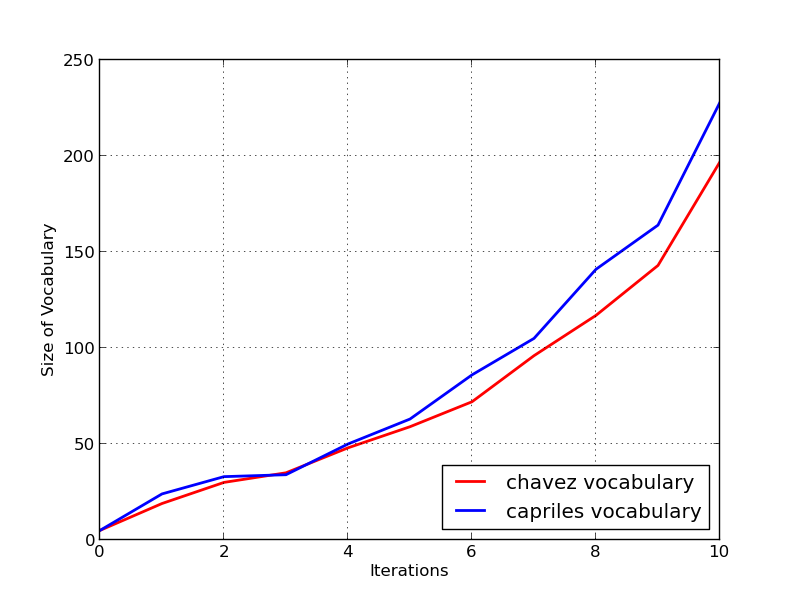
\includegraphics[scale=0.50]{support_files/WordGrowth.png}
	\caption{Vocabulary growth with each iteration.}
	\label{fig:wordgrowth}
\end{figure*}
For tweets that do not have a positive or negative orientation we assign a truth value of $0.5$ for both the $Positive$ and $Negative$ predicates.\\
The last two rules defined below encode the assumption that when two hash-tags co-occur and one is a name of a candidate then the other hash-tag is bound to be about the candidate too.
\begin{align*}
\begin{split}
Contains(T,W1)
 \softand Contains(T,W2)
  \softand Seed\_Word(W1,G)\\ 
  \softand Positive(T)
	\Rightarrow Belongs(W2,G)
\end{split}
\end{align*}

\begin{align*}
\begin{split}
Contains(T,W1) 
	\softand Contains(T,W2)
	\softand Seed\_Word(W1,G)\\ 
	\softand Negative(T)
	\Rightarrow \sim Belongs(W2,G)
\end{split}
\end{align*}
Once all the tweets are loaded into the PSL program as predicates, we start the inference process by closing all the predicates except $Is\_Member$ and $Belongs$. 
This way, only their truth values are inferred.
\section{Results}
\begin{figure*}
	\centering
	\subfloat[Day 0]
	{
		
\includegraphics[width=0.5\textwidth, height=0.20\textheight]{support_files/caprilesWordCloud1.png}
		\label{fig:wordCloud1}
	} 
	\subfloat[Day 6]
	{
		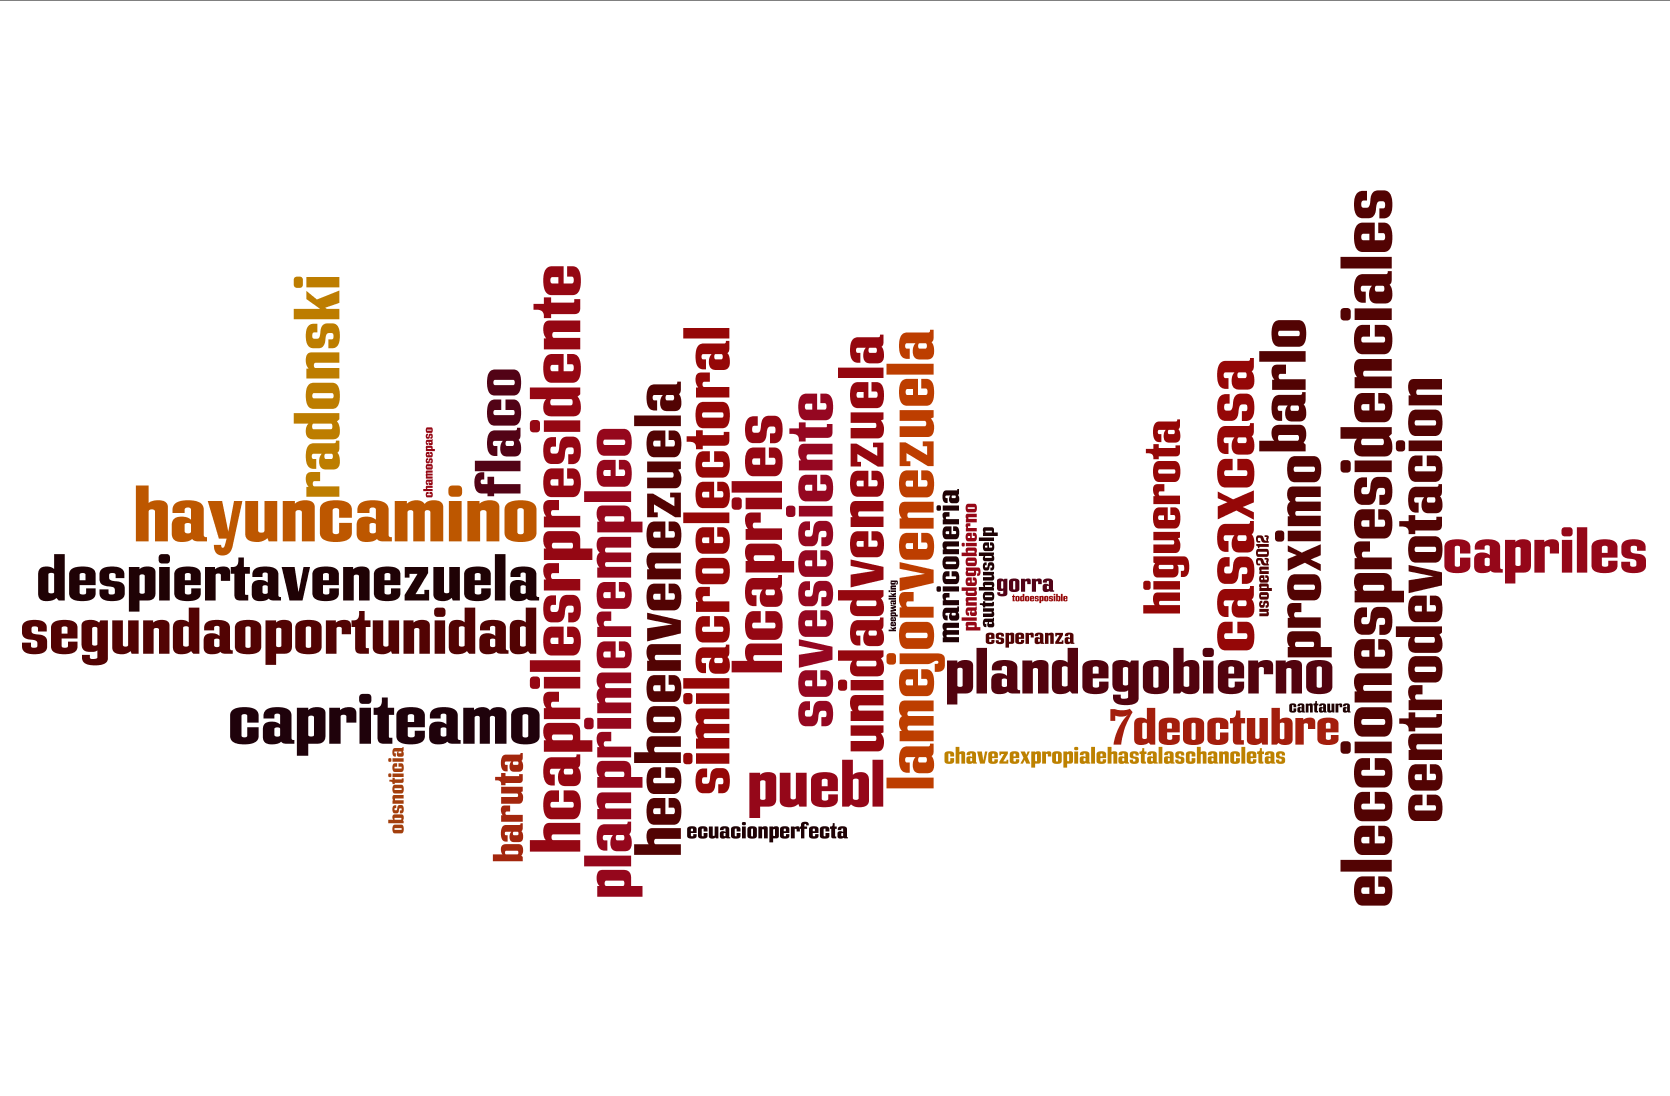
\includegraphics[width=0.5\textwidth, height=0.20\textheight]{support_files/caprilesWordCloud2.png}
		\label{fig:wordCloud2}
	} \\
	\noindent 
	\subfloat[Day 15]
	{
		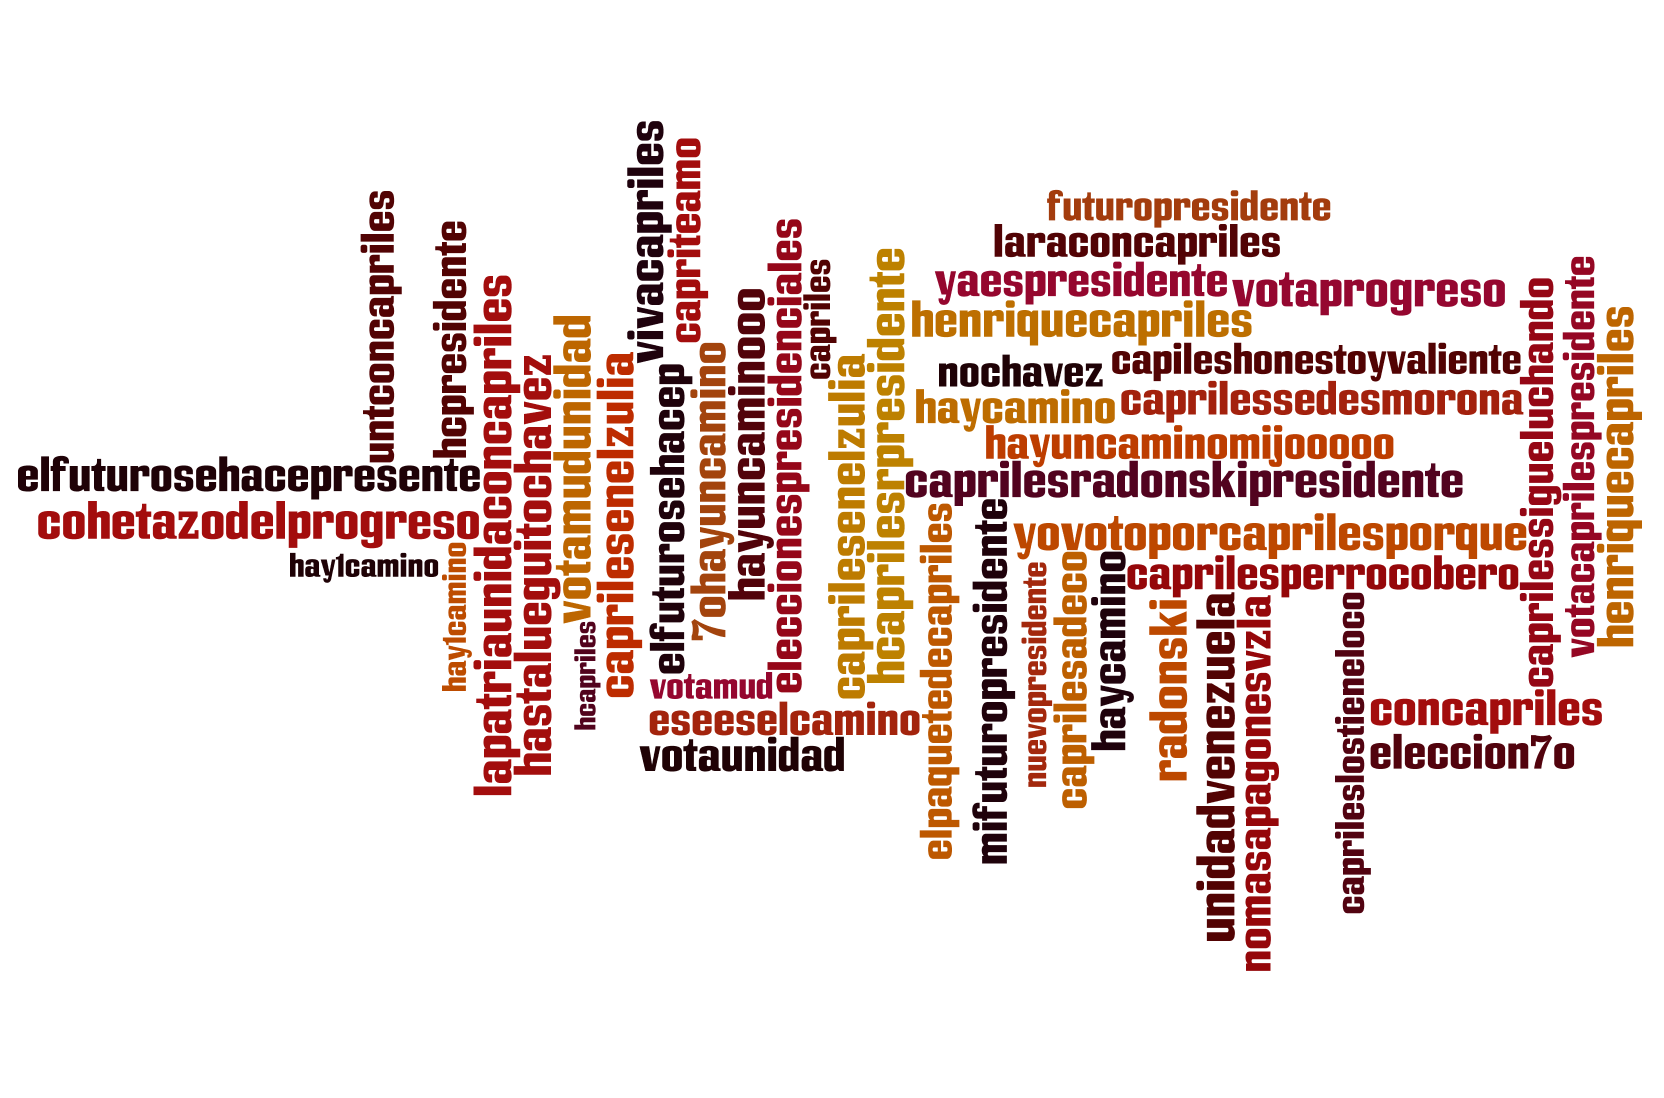
\includegraphics[width=0.5\textwidth, height=0.20\textheight]{support_files/caprilesWordCloud3.png}
		\label{fig:wordCloud3}
	}
	\subfloat[Day 30]
	{
		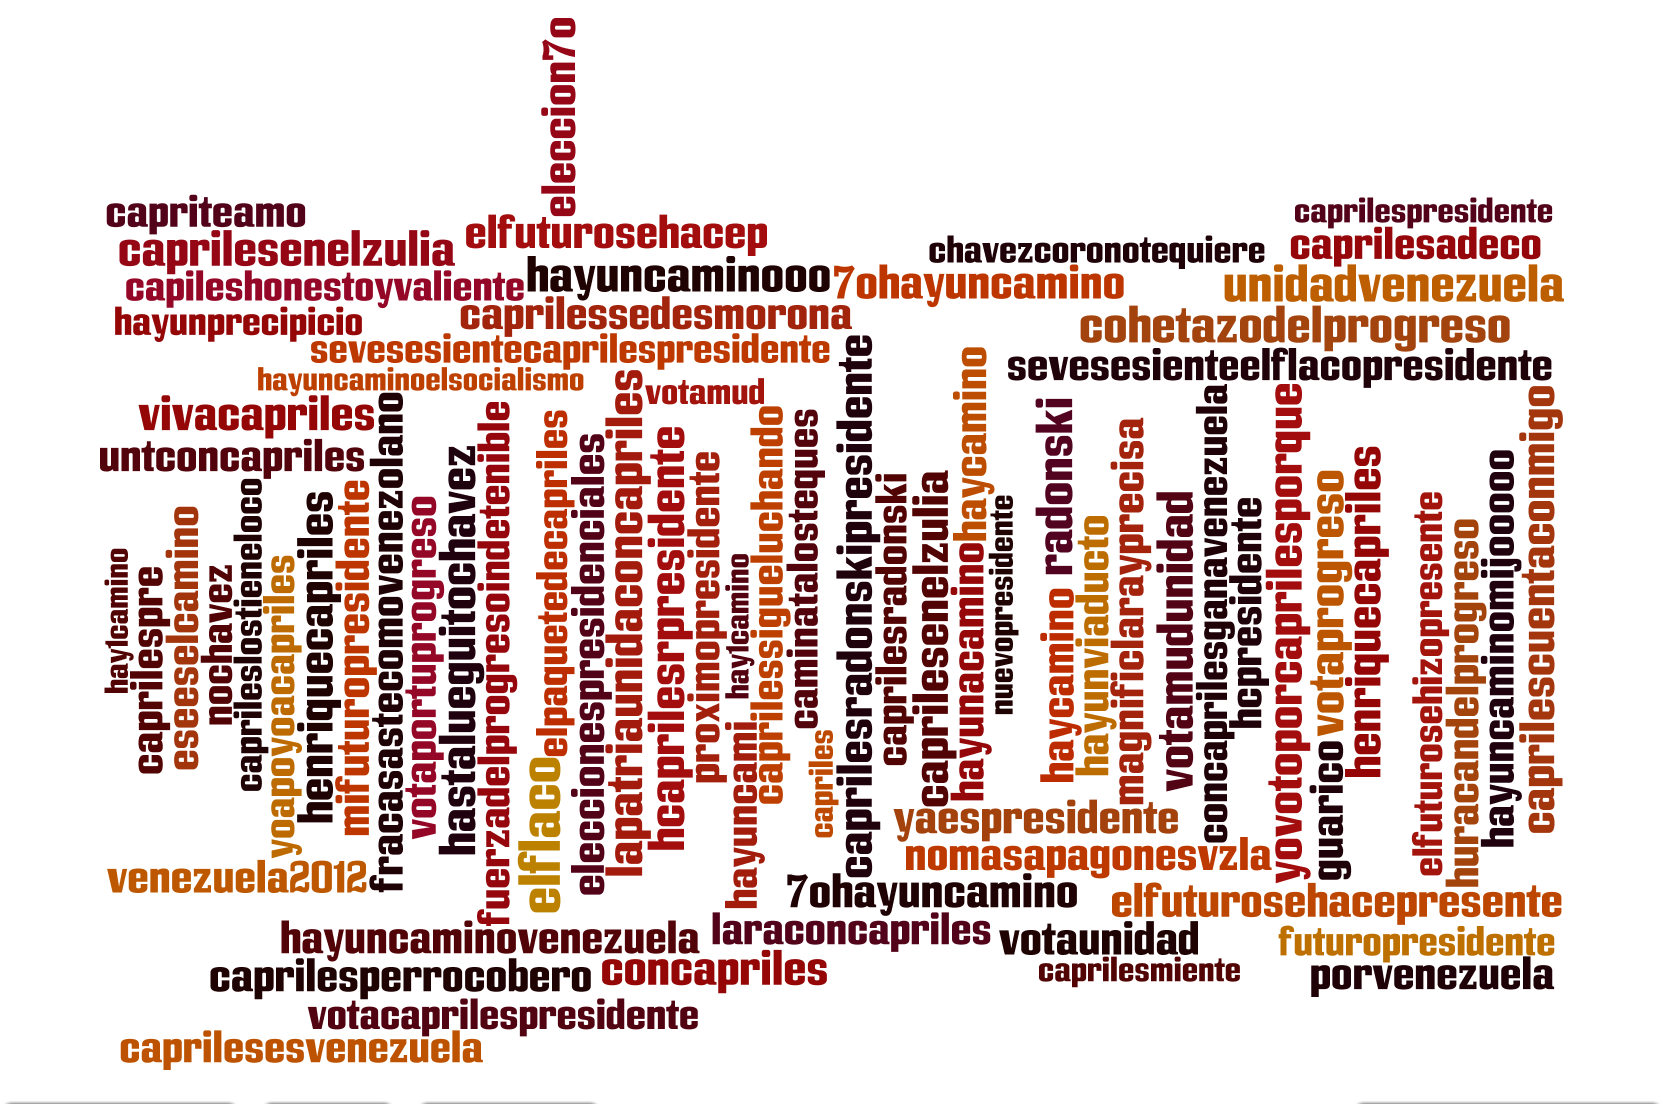
\includegraphics[width=0.5\textwidth, height=0.20\textheight]{support_files/caprilesWordCloud4.png}
		\label{fig:wordCloud4}
	}
	\caption{Evolution of hash-tags for Henrique Capriles} 
	\label{fig:wordCloud}
\end{figure*}

Figure\ref{fig:wordgrowth} shows  how the vocabulary grows with each iteration for the two candidates who contested the Venezuelan presidential election on October 7th 2012.\\
Figure\ref{fig:wordCloud} shows how the hash-tags for Henrique Capriles evolved during the month leading up to the election.
Initially in Figure\ref{fig:wordCloud1} the system starts with only a few hand picked hash-tags that constitute the seed vocabulary. 
After a few iterations Figure\ref{fig:wordCloud2} shows how the vocabulary has grown.
However, not all the words identified until now remain in the final vocabulary as the system drops certain words in successive iterations.
At the same time it is also noticed that hash-tags like "capriles" and "hayuncamino" which are very strongly associated with Capriles consistently remain as the top ranked hash-tags even after ten iterations(Figure\ref{fig:wordCloud4}). 
It is also interesting to note that the algorithm identified hash-tags like "nochavez"(Figure\ref{fig:wordCloud3}) and attributed it rightly to Hugo Chavez's primary contender- Capriles. \\
\begin{figure*}[Ht]
	\centering
	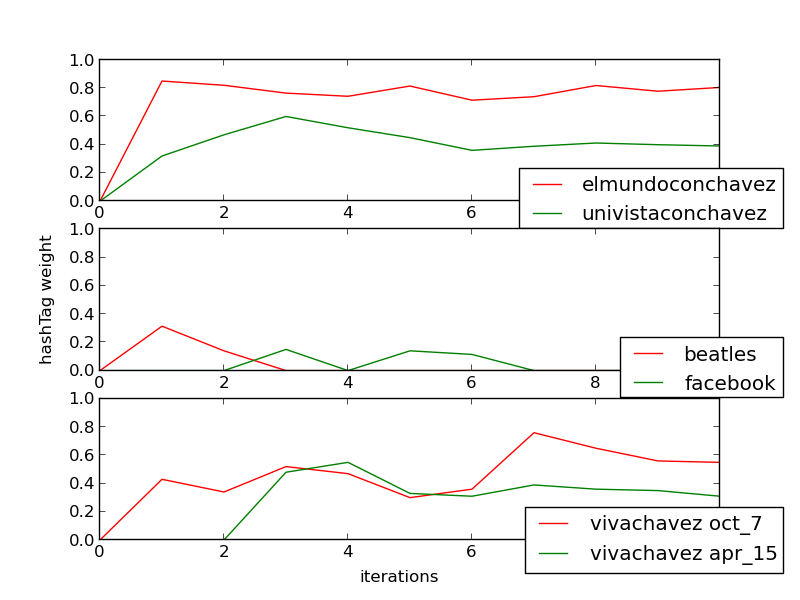
\includegraphics[scale=0.65]{support_files/hashTagTimeSeries.png}
	\caption{Time series comparison for different hash-tags identified for Hugo Chavez.}
	%The first plot shows "univistaconchavez" and "elmundocochavez". The second plot shows "Beatles" and "Facebook". The third plot shows "vivachavez" from two different elections conducted on 15th April 2013 and 7th October 2012.
	\label{fig:timeSeries}
\end{figure*}
In figure \ref{fig:timeSeries}, the first plot elucidates how hash-tags like \emph{"elmnduconchavez"} and \emph{"univistaconchavez"} remain highly associated with Hugo Chavez for the October 7th Presidential election. 
These hash-tags remain indicative of a user's affiliation throughout the month leading up to the election.
Meanwhile hash-tags such as \emph{"beatles"} and \emph{"facebook"} ( in second plot) show spikes in their time series primarily because users affiliated with Chavez used them during that time window. 
But as iterative process continues the system drops these non-informative words.
The third plot presents another interesting observation 
The hash-tag \emph{"vivachavez"} is part of both the Venezuelan elections despite the fact that Hugo Chavez did not contest the second election on April 15th 2013. 
It is picked up as a phrase commonly used by supporters of Nicholas Maduro whose election campaign was strategized around the death of Hugo Chavez to garner sympathy and mobilize support.
Similarly variations of the hash-tags \emph{"hayuncamino"} and \emph{"unidadvenuzela"} was returned for Henrique Capriles for both these elections.